% Chapter 1

\chapter{Introducción General} % Main chapter title

\label{Chapter1} % For referencing the chapter elsewhere, use \ref{Chapter1} 
\label{IntroGeneral}

%----------------------------------------------------------------------------------------

% Define some commands to keep the formatting separated from the content 
\newcommand{\keyword}[1]{\textbf{#1}}
\newcommand{\tabhead}[1]{\textbf{#1}}
\newcommand{\code}[1]{\texttt{#1}}
\newcommand{\file}[1]{\texttt{\bfseries#1}}
\newcommand{\option}[1]{\texttt{\itshape#1}}
\newcommand{\grados}{$^{\circ}$}

%----------------------------------------------------------------------------------------

%\section{Introducción}

%----------------------------------------------------------------------------------------
\section{Descripción general del trabajo y conceptos claves}

El trabajo desarrollado consiste en un sistema adquisidor de datos con los sensores necesarios para una medición de potencia eléctrica, en otras palabras un medidor digital de energía eléctrica. El trabajo fue desarrollado para una empresa privada localizada en Argentina.

Las mediciones eléctricas son los métodos, dispositivos y cálculos usados para medir cantidades eléctricas. La medición de cantidades eléctricas puede hacerse al medir parámetros eléctricos de un sistema. Usando transductores, propiedades físicas como la temperatura, presión, flujo, fuerza, y muchas otras pueden convertirse en señales eléctricas, que pueden ser convenientemente registradas y medidas. 

%\citep{MEcitation}

La adquisición de datos o adquisición de señales consiste en la toma de muestras del mundo real (sistema analógico) para generar datos que puedan ser manipulados por un ordenador u otros dispositivos electrónicos (sistema digital). Se requiere una etapa de acondicionamiento, que adecua la señal a niveles compatibles con el elemento que hace la transformación a señal digital.\cite{NIDataAdquisition}

\begin{figure}[h]
	\centering
	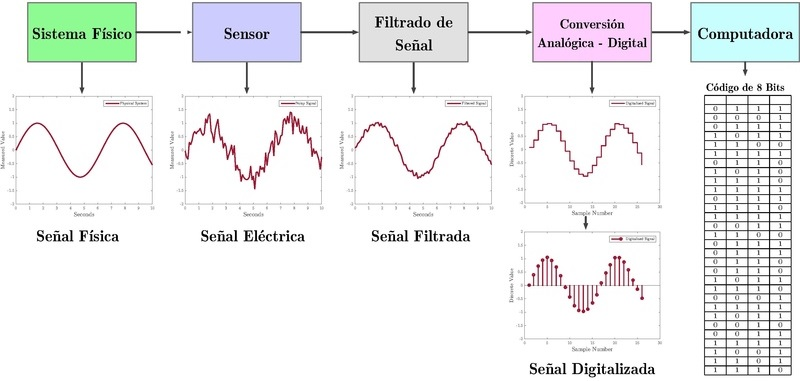
\includegraphics[width=120mm,keepaspectratio]{Figures/DigitalDAQ.jpg}
	\caption{Ejemplo de digitalización de una señal.}
	\label{fig:texmaker}
\end{figure}

Un convertidor de señal analógica a digital (ADC) es un dispositivo electrónico capaz de convertir una señal analógica, ya sea de tensión o corriente, en una señal digital mediante un cuantificador y codificándose en muchos casos en un código binario en particular. 
%\citep{ADCcitation}

\subsection{Sistemas electrónicos para mediciones eléctricas}

Las aplicaciones mas tempranas de computadores digitales a problemas de sistemas de potencia datan alrededor de 1940. La mayoría de las aplicaciones tempranas estaban limitadas en alcance debido a la pequeña capacidad de las tarjetas calculadoras usadas en ese periodo. Computadoras digitales de larga escalas estuvieron disponibles a mediados de 1950, y el éxito inicial de programas de flujo de carga llevaron al desarrollo de programas para cálculos de corto circuitos y estabilidad.\citep{761852}

Los medidores electrónicos digitalizan las variables medidas vía un ADC sigma delta  de alta resolución. La técnica de diseño de estos medidores digitales es influenciada por tres grandes factores: el costo , eficiencia y tamaño. Mientras que el costo esta influenciado por la capacidad de compra del cliente, la eficiencia y el tamaño deben cumplir estrictamente con los estándares.\cite{articleDM}

\begin{figure}[h]
	\centering
	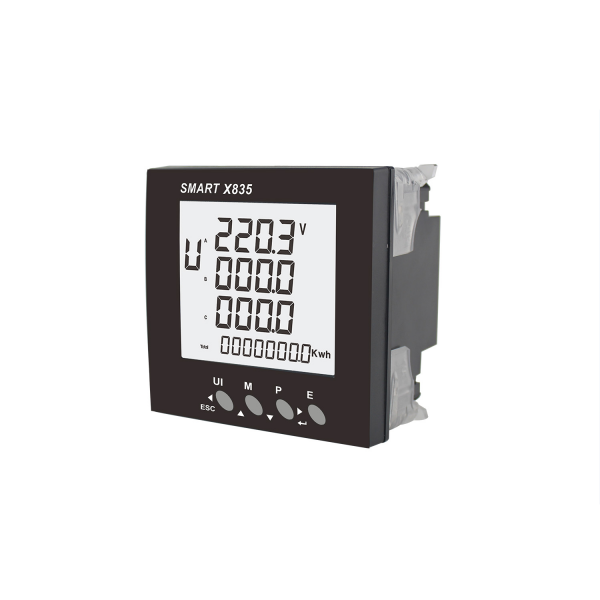
\includegraphics[width=55mm,keepaspectratio]{Figures/3931_1.png}
	\caption{Medidor electrónico comercial.}
	\label{fig:texmaker}
\end{figure}

La exactitud del medidor eléctrico digital depende en la exactitud del circuito analógico de entrada analógica, la exactitud del conversor analógico-digital y la exactitud de los cálculos digitales.\citep{Hribik2004DigitalPA}

Los convertidores analógicos-digitales basados en la modulación sigma - delta son económicamente viables para convertidores de alta resolución (mayores que 12bits), por lo que son  usados en el circuito integrado de procesadores de señales.

La modulación sigma-delta fue introducida en 1962 y no ganaría importancia hasta recientes desarrollos en tecnologías VLSI(integración a escala muy grande) que proveían fines prácticos para implementar complejos circuitos de procesamiento de señales.\citep{book:28601}


%%

\section{Motivación}

En la actualidad se pueden encontrar en el mercado internacional múltiples módulos electrónicos, de bajo costo, con puertos de comunicación para la medición de energía eléctrica como así también medidores digitales de energía de diferentes marcas para diferentes entornos, los que nos permite pensar que un dispositivo similar podría ser fabricado en la Argentina.

\begin{figure}[h]
	\centering
	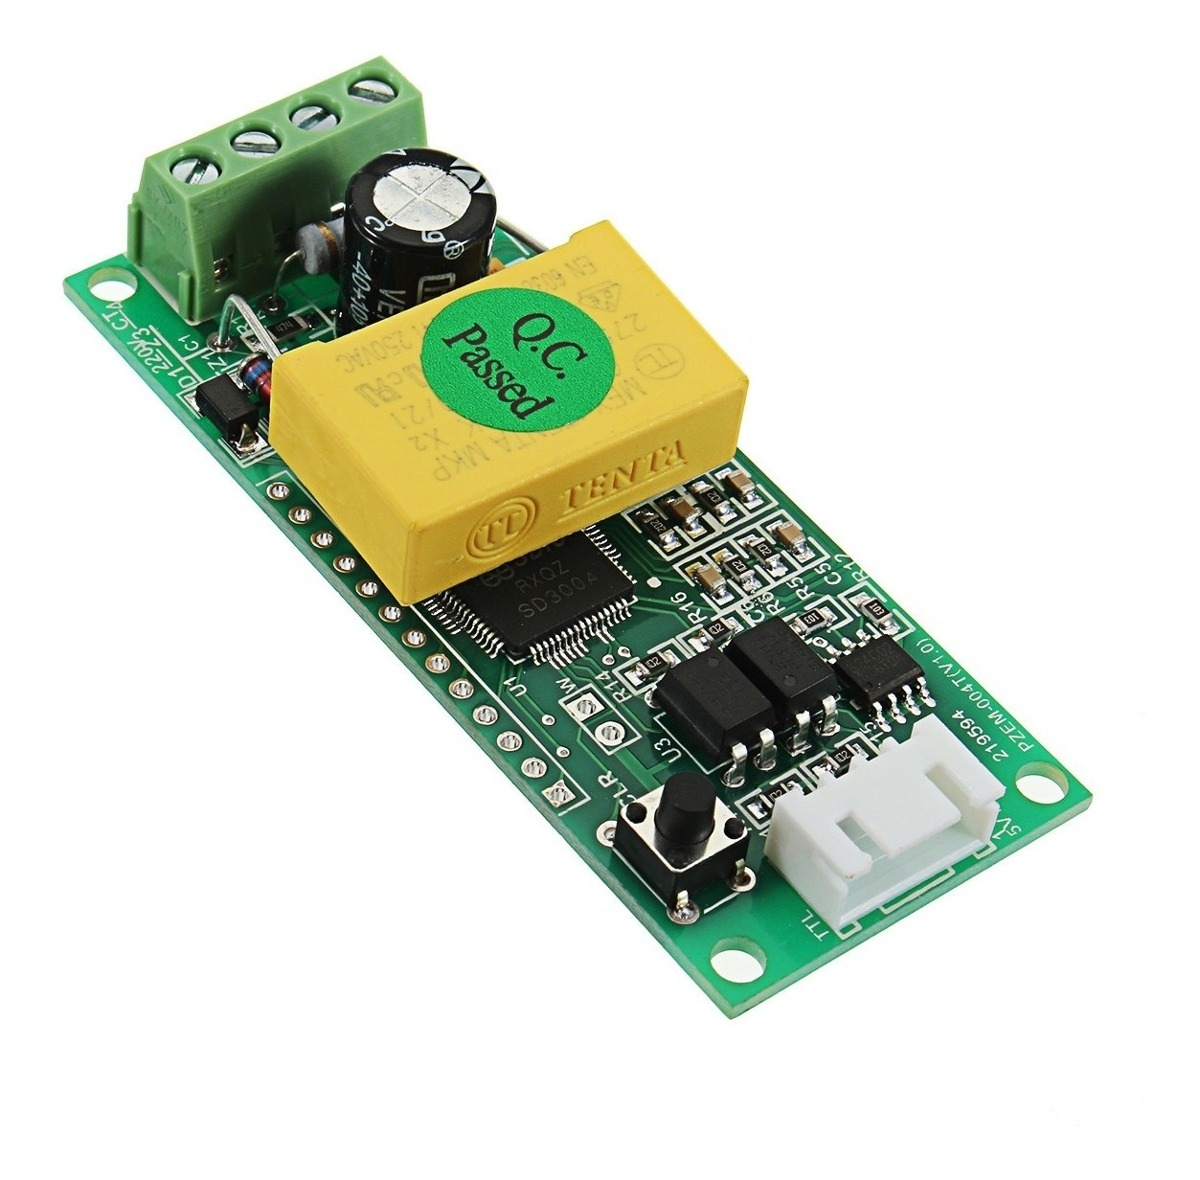
\includegraphics[width=80mm,keepaspectratio]{Figures/pzeem004.jpg}
	\caption{Modulo de medición de energía eléctrica con comunicación serie universal.}
	\label{fig:pzem04}
\end{figure}

Los módulos de medición pueden servir como un monitoreo de primera instancia pudiendo ser un método preventivo de fallas, dado que los parámetros de consumo dan una idea de estado de las máquinas.  El módulo de la figura \ref{fig:pzem04}  anterior fue usado en un trabajo de grado para un local comercial cuyo resultados pueden verse en la figura \ref{fig:graficoW}.  Estas gráficas sirvieron para realizar observaciones como el encendido de un motor trifásico y mal-funcionamiento de equipos de refrigeración.

\begin{figure}[h]
	\centering
	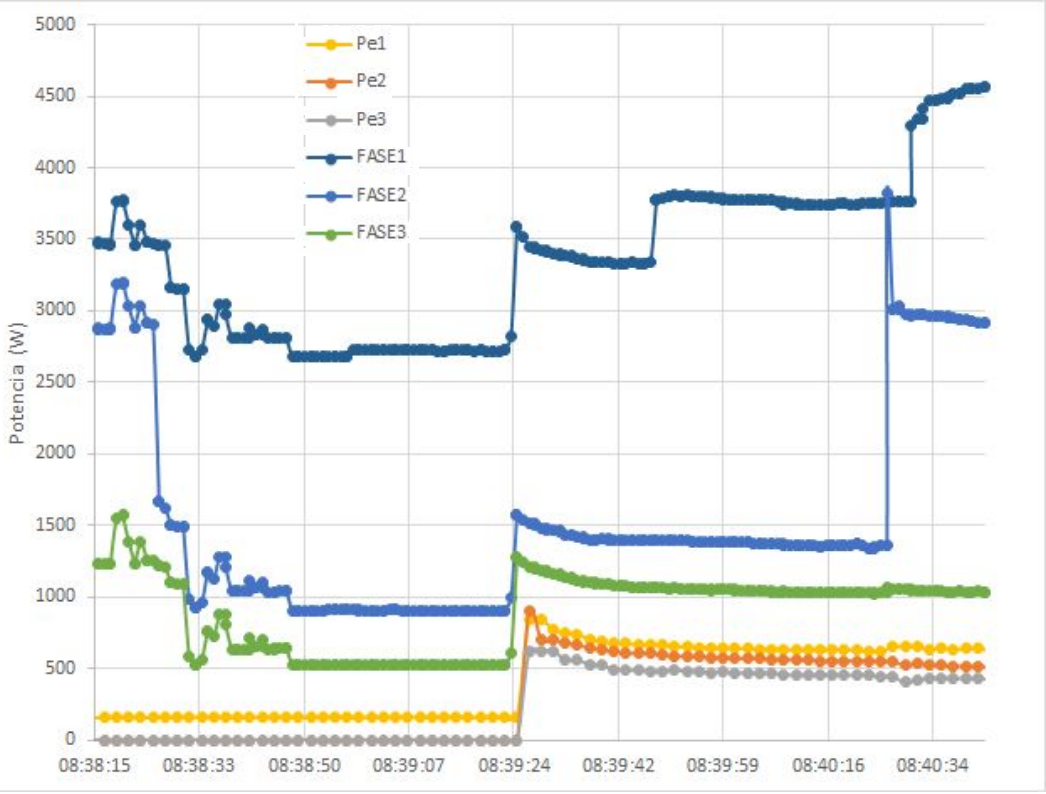
\includegraphics[width=80mm,keepaspectratio]{Figures/potencia_ej.png}
	\caption{Gráfico de medición de potencia mostrando el encendido de un frigorífico.}
	\label{fig:graficoW}
\end{figure}

Estos módulos se consiguen en el mercado internacional de modo que hay que importarlos lo que presenta una barrera para una herramienta de monitoreo simple. 

Desde el punto de vista de la empresa privada  el trabajo se planteó ante la necesidad de cuantificar consumos energéticos de procesos industriales para supervisar la alimentación de equipos de control o de medición. También como una alternativa a un producto anterior que solo media consumos de corriente continua. 

Por lo que la necesidad de hacer uso de la herramienta y la capacidad de realizar la electrónica de manera local  fueron los impulsores del trabajo realizado.

\section{Objetivos y alcance}

\subsection{Objetivos del desarrollo}
El objetivo del proyecto es el desarrollo de un dispositivo de medición, basado en un un micro-controlador de la familia MSP430 en conjunto con un ADC SOC(system on chip). Se pretende lograr un dispositivo comercial similar a aquellos elaborados anteriormente por la empresa privada, por lo que las dimensiones del PCB (printed circuit board) deberán ajustarse a los utilizados por las carcasas estándar que utiliza la empresa, como puede verse en la figura \ref{fig:disp_emp}.

\begin{figure}[h]
	\centering
	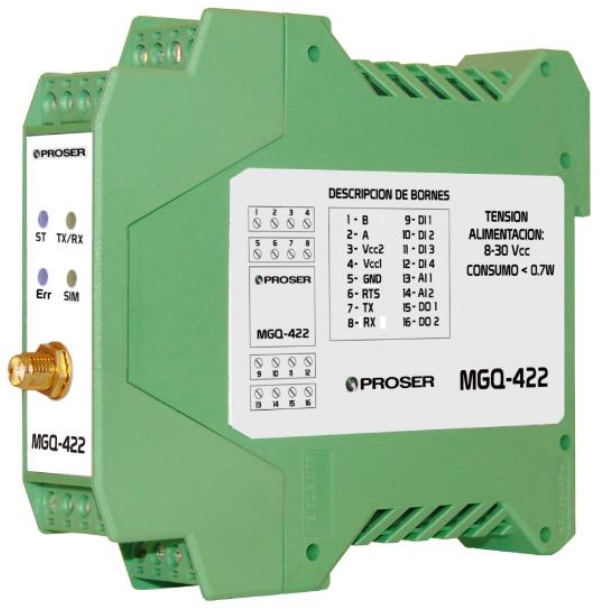
\includegraphics[width=80mm,keepaspectratio]{Figures/dispositivo_empresa.png}
	\caption{Ejemplo de dispositivo fabricado por la empresa privada.}
	\label{fig:disp_emp}
\end{figure}

Además se espera que el firmware maneje protocolo modbus y comunique las variables medidas a través de los puertos de comunicación. Físicamente se espera que el dispositivo sea capaz de comunicar por puertos serie RS-232 y RS-485, y ser diseñado pensando en su uso industrial (el dispositivo deberá ser robusto).


\subsection{Alcances}


%----------------------------------------------------------------------------------------

El trabajo abarca desde el planteo, diseño y fabricación de un pcb, la selección de componentes la elaboración del esquemático de conexiones lógicas, elaboración del pcb y su diseño teniendo en cuenta la fabricación de este hasta inclusive la elaboración de un prototipo y testeo sobre este.

También se espera que se  realice un firmware para el funcionamiento del dispositivo, teniendo en cuenta que el software debe incluir métodos de configuración para un futuro usuario.





